% Testing Chapter

%% FIXME: Case study 1 (What, how, )

%%  * Describe test setup
%%  * For each case study - test case
%%  * Experiment -
%%    * clearly described test aim (What?)
%%    * How / What are the specifics of this test case / case study?
%%    * RESULTS
%%    * ANALYSIS


\section{Case Study 1: Identify Protocols}
\label{sec:casestudy1}

\subsection{What was studied}

The purpose of this case study is to identify network protocols used
in online installation infrastructure system. This study also verifies
the involved protocols which were described in the introduction
chapter.

For installation infrastructure a service called
boot.foo.sh~\cite{boot-foo-sh} is used. Boot.foo.sh was chosen because
it's open service known to be used to automatic installations in
enterprises and it has been an inspiration to this thesis to make
installation infrastructure more safer to use.

Boot.foo.sh is used to install CentOS~7 Linux operating system. CentOS
Linux is community driven effort to provide free alternative to Red
Hat Enterprise Linux (RHEL). CentOS is built using RHEL source
code. Red Hat has 67 \% market share of Linux distribution market
according to Gartner's analysis~\cite{gartner-redhat}.

\subsection{How it was done}

The installation was done using virtual machine. VirtualBox was chosen
as a virtualization software because it's free, open source and has
easy to use network traffic recording functionality.

\begin{figure}[h]
  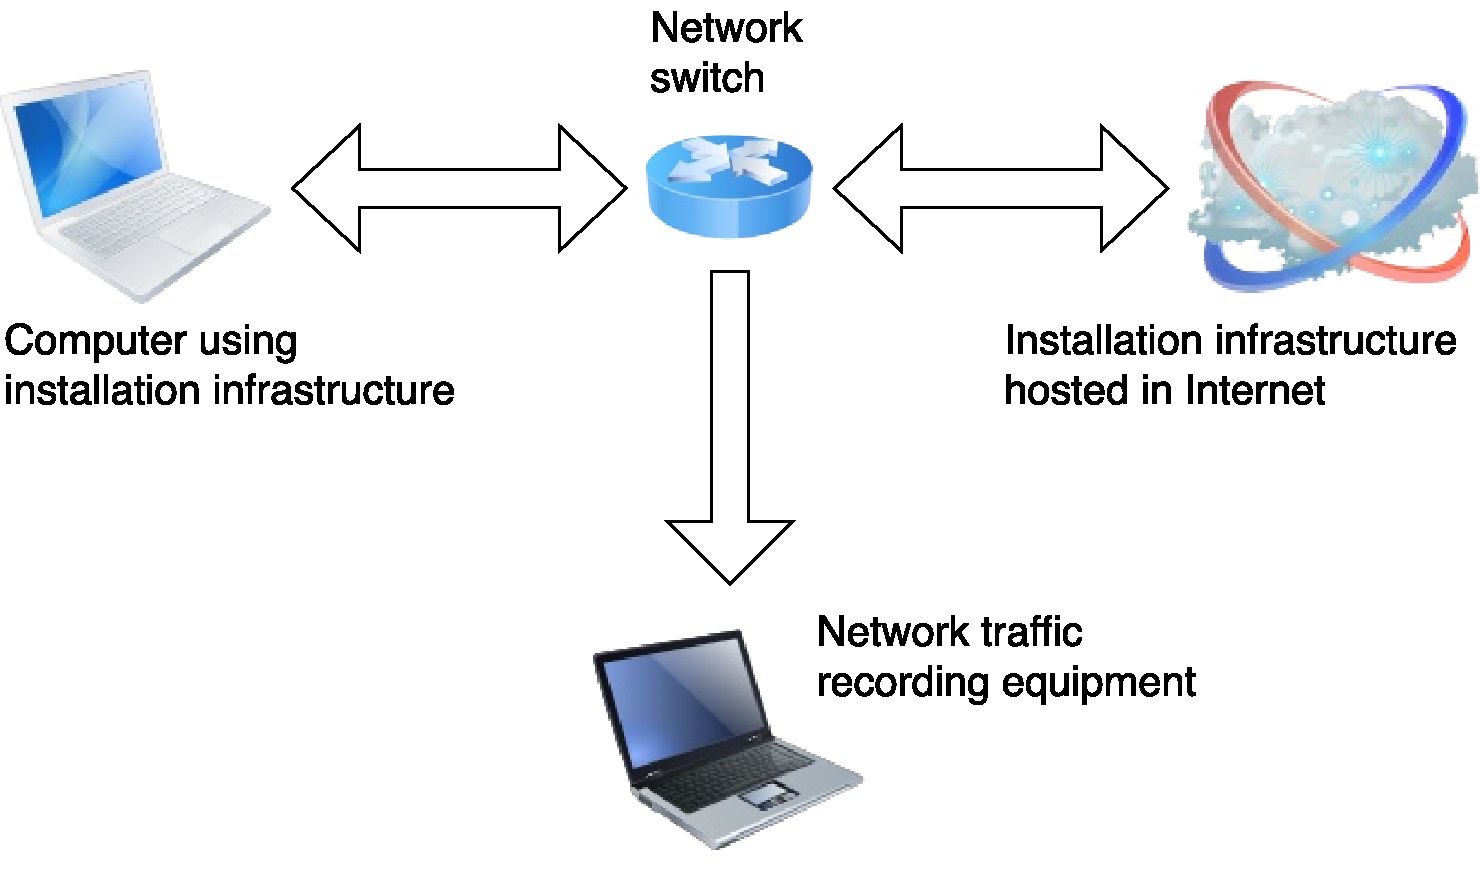
\includegraphics[width=\textwidth]{network-recording.pdf}
  \caption{Network traffic recording setup.\label{fig:network-recording}}
\end{figure}

With VirtualBox's network traffic recording it's possible to get
network traffic captured for the whole lifetime of virtual
machine. The capture is saved as standard PCAP file which can later be
opened in network protocol analyzer for
investigation. Figure~\ref{fig:network-recording} has the typical
traffic capturing setup with computer using the installation
infrastructure, another computer recording the traffic, network switch
to arrange traffic flows and the Internet containing the installation
infrastructure in use.

Traffic capture was then analyzed using Wireshark network protocol
analyzer. Wireshark is free and open source network protocol analyzer
which has capability to help expert user analyze many different
network protocols and their internals.

Traffic analysis was done by hand looking the captured traffic
recording and identifying protocols used.

\subsection{Results found}

Traffic recording was 788 megabytes of network traffic containing over
883 thousand network packets. Recording contains time span of a bit
over nine minutes.

\begin{table}[!ht]
  % Add some padding to the table cells:
  \def\arraystretch{1.1}%
  \begin{center}
    \begin{tabular}{| l | l |}
      \hline
      Step               & protocol    \\
      \hline
      Address resolution & DHCP        \\
      Name resolution    & DNS         \\
      Boot menu          & HTTPS       \\
      kernel and initrd  & HTTP        \\
      Kickstart          & HTTP        \\
      Installation files & HTTP (DS)   \\
      \hline
    \end{tabular}
    \caption{Table of found protocols and their role. DS in table
      means Digital Signatures.\label{tab:found_protocols_table}}
  \end{center}
\end{table}

Summary of the protocols used in various steps of installation process
can be found from Table~\ref{tab:found_protocols_table}.

Steps are identified and named for each system used to achieve the
installation. The steps are discussed in chronological order of
appearance as found from traffic recording.

\subsection{Analysis of results}

``Address resolution'' is the first step and it's purpose is to get IP
address and DNS server addresses for system to be installed. DHCP is
the standard protocol for this, and was also found to be used here.

``Name resolution'' is used to translate host names into IP address to
communicate with other servers. DNS protocol is used for name
resolution needs.

\begin{figure}[h]
  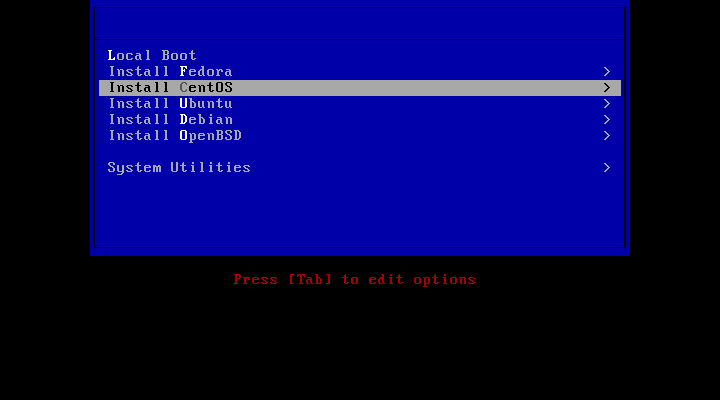
\includegraphics[width=\textwidth]{bootfoosh-bootmenu.png}
  \caption{boot.foo.sh boot menu showing selection of operating
    systems.\label{fig:bootmenu}}
\end{figure}

``Boot menu'' is used to display choices of operating systems to be
installed. Boot menu from boot.foo.sh can be seen in
figure~\ref{fig:bootmenu}. Boot.foo.sh uses HTTP protocol to fetch
various files needed to display the boot menu.

``kernel and initrd'' are the files needed to launch Linux
installation. These two files are downloaded over the Internet and
then kernel is executed and it continues the boot process. HTTP was
used to communicate with CentOS 7 mirror to fetch the needed files.

``Kickstart'' is CentOS specific file for automating unattended
installation. It's set of instructions downloaded and executed by the
installation process. Kickstart file is downloaded by software inside
initrd system so at this point the control of installation is already
switched to CentOS' installer. HTTP was used to communicate with
boot.foo.sh server to fetch the kickstart file.

``Installation files'' are the contents of operating system to be
installed. The files are downloaded and extracted to hard drive to
achieve the installation. Operating system installer is usually
trusted to verify digital signatures (e.g. CentOS uses
OpenPGP~\cite{RFC4880} (``GPG'') signatures) the downloaded content
before extracting the files into hard drive. The CentOS
documentation~\cite{centos-gpg} states that

\begin{quote}
Each stable RPM package that is published by CentOS Project is signed
with a GPG signature. By default, yum and the graphical update tools
will verify these signatures and refuse to install any packages that
are not signed, or have an incorrect signature. You should always
verify the signature of a package prior to installation. These
signatures ensure that the packages you install are what was produced
by the CentOS Project and have not been altered by any mirror or
web site providing the packages.
\end{quote}

However, when initrd file is downloaded over insecure protocol or file
content is not verified against signature it's possible for malicious
third party to inject it's own OpenPGP keys into initrd and point
installation system to malicious host serving the operating system
installation files and thus gain full control of the installed system.


\section{Case Study 2: Comparing boot.foo.sh and secudep}
\label{sec:casestudy2}

\subsection{What was studied}

Compare results from case study 1 to how secudep works.

\subsection{How it was done}



\subsection{Results found}

\begin{table}[!ht]
  % Add some padding to the table cells:
  \def\arraystretch{1.1}%
  \begin{center}
    \begin{tabular}{| l | l | l |}
      \hline
      Step               & boot.foo.sh   & secudep    \\
      \hline
      Address resolution & DHCP          & DHCP       \\
      Name resolution    & DNS           & DNS        \\
      Boot menu          & HTTP          & HTTPS (DS) \\
      Digital signatures & N/A           & HTTPS      \\
      kernel and initrd  & HTTP          & HTTP (DS)  \\
      Kickstart          & HTTP          & HTTPS      \\
      Installation files & HTTP (DS)     & HTTP (DS)  \\
      \hline
    \end{tabular}
    \caption{Comparison between how boot.foo.sh and secudep use of
      protocols. DS in table means Digital
      Signatures.\label{tab:comparison_table}}
  \end{center}
\end{table}

Results of comparing boot.foo.sh and secudep can be found from
Table~\ref{tab:comparison_table}. Boot.foo.sh results are same as in
case study 1.

The differences between boot.foo.sh and secudep in
Table~\ref{tab:comparison_table} are discussed next.

''Boot menu'' is used to display choices of operating systems to be
installed. HTTP is used in boot.foo.sh. HTTP protocol is susceptible
to Man in the Middle attack. Secudep uses HTTPS (HTTP over TLS) with
signed files to redemiate this issue.

\begin{figure}[h]
  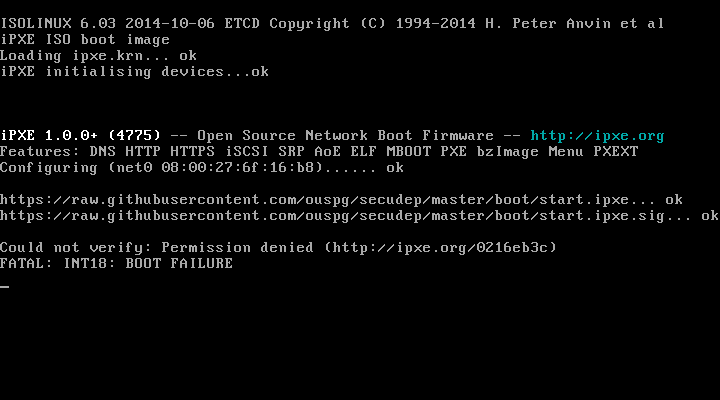
\includegraphics[width=\textwidth]{verify-fail.png}
  \caption{Installation process is halted when digital signature
    verification fails.\label{fig:verify-fail}}
\end{figure}

Only secudep uses digital signatures and the signature files are
fetched over HTTPS.\@ This is a step missing from
boot.foo.sh. Figure~\ref{fig:verify-fail} shows how secudep's process
is halted when the digital signature verification fails. This failure
is a clear indication that something is wrong.

Kernel and initrd are the files needed to launch the Linux
installation. Both boot.foo.sh and secudep systems use HTTP
protocol. Again HTTP is susceptible to Man in the Middle attacks. HTTP
is used because the files are fetched from CentOS's official mirror
over the internet. Secudep uses digital signatures to verify
downloaded content. After kernel and initrd are downloaded and digital
signatures are verified the execution is handled to kernel. This means
that secudep can't provide digital signatures to any following files.
